\section{Results}\label{sec:results}
The longitudinal study commenced in April 2020 and ended in December 2020 in Singapore.
A total of 20 participants (10 males and 10 females) took part in our study.
Key information about each participant is presented in Table~\ref{tab:subject_info}.

\begin{table}[h!]
\centering
\caption{Information about the subjects.}
\label{tab:subject_info}
\small \begin{tabular}{cccccccccccccccc}
\toprule
 ID & Sex &  Age &            Education &  BMI (kg/m$^{2}$) \\
\midrule
  1 &   M &   38 &      Doctoral degree &             23.51 \\
  2 &   M &   36 &      Doctoral degree &             29.40 \\
  3 &   M &   30 &      Doctoral degree &             25.54 \\
  4 &   F &   40 &      Master's degree &             18.29 \\
  5 &   M &   31 &      Doctoral degree &             25.39 \\
  6 &   M &   44 &      Doctoral degree &             21.22 \\
  7 &   F &   30 &    Bachelor's degree &             25.93 \\
  8 &   M &   35 &      Doctoral degree &             25.10 \\
  9 &   F &   24 &      Master's degree &             23.24 \\
 10 &   M &   24 & High school graduate &             23.05 \\
 11 &   F &   29 &      Master's degree &             20.20 \\
 12 &   M &   34 &      Doctoral degree &             28.20 \\
 13 &   M &   31 &    Bachelor's degree &             25.34 \\
 14 &   M &   35 &    Bachelor's degree &             23.03 \\
 15 &   F &   33 &      Doctoral degree &             18.34 \\
 16 &   F &   26 &    Bachelor's degree &             20.45 \\
 17 &   F &   36 &      Doctoral degree &             18.37 \\
 18 &   F &   26 &    Bachelor's degree &             22.04 \\
 19 &   F &   24 &    Bachelor's degree &             16.44 \\
 20 &   F &   32 &      Doctoral degree &             20.96 \\
\bottomrule
\end{tabular}
\end{table}


\subsection{Dataset preparation and cleaning}\label{subsec:datasetPreparationAndCleaning}
Participants completed a total of \var{tot_surveys} \ac{rhrn}.
Of the total surveys collected, participants completed \var{per_surveys_exercising}~\% of them while exercising, \var{per_surveys_outdoor}~\% while outdoors, and \var{per_surveys_change}~\% while in transitory conditions.
These surveys were not included in the data analysis as previously explained in Section~\ref{subsubsec:data-preparation}.

The \ac{t-sk-w} and \ac{t-nb} data we measured while the participants completed the \ac{rhrn} are depicted in Figure~\ref{fig:tmp_skin_nb_survey}a\@.
In approximately 97~\% of the total completed surveys, the value of \ac{t-sk-w} was higher than \ac{t-nb}.
This result was expected since the maximum value of \ac{t-db} that participants experienced throughout the study never exceeded 34~$^{\circ}$C\@.
For example, the delta between \ac{t-sk-w} and \ac{t-nb} in participant 10 was as low as \var{diff_tnb_tsk_user_10}~$^{\circ}$C\@, while the average value across all participants was \var{mean_diff_tnb_tsk}~$^{\circ}$C\@.
We consequently remove the data using the methodology detailed in Section~2 of the Appendix.
This removed more than 15~\% of the total number of surveys collected by the following participants 05, 10 (73~\% excluded), 12, 14, and 18.

This sub-set of the original dataset, which included \var{tot_surveys_filtered} survey responses, was used in the data analysis.
The filtered number of surveys for each participant is shown in Figure~\ref{fig:tmp_skin_nb_survey}~b\@.

\subsection{Dataset overview}\label{subsec:datasetOverview}
The \var{tot_surveys_filtered} survey responses are summarized in Figure~\ref{fig:ans_distribution}.
Votes in Q.1--`Thermal preference' were mostly `No Change' (\var{per_no_change}~\%) followed by `Cooler' (\var{per_cooler}~\%).
This study took part during the COVID-19 pandemic, and most of the participants had to work from home for the whole study duration.
Participants in their homes had full control of the air-conditioning set-point and could use electric fans to increase airspeed in their surroundings.

\begin{figure}[thb!]
     \begin{center}
         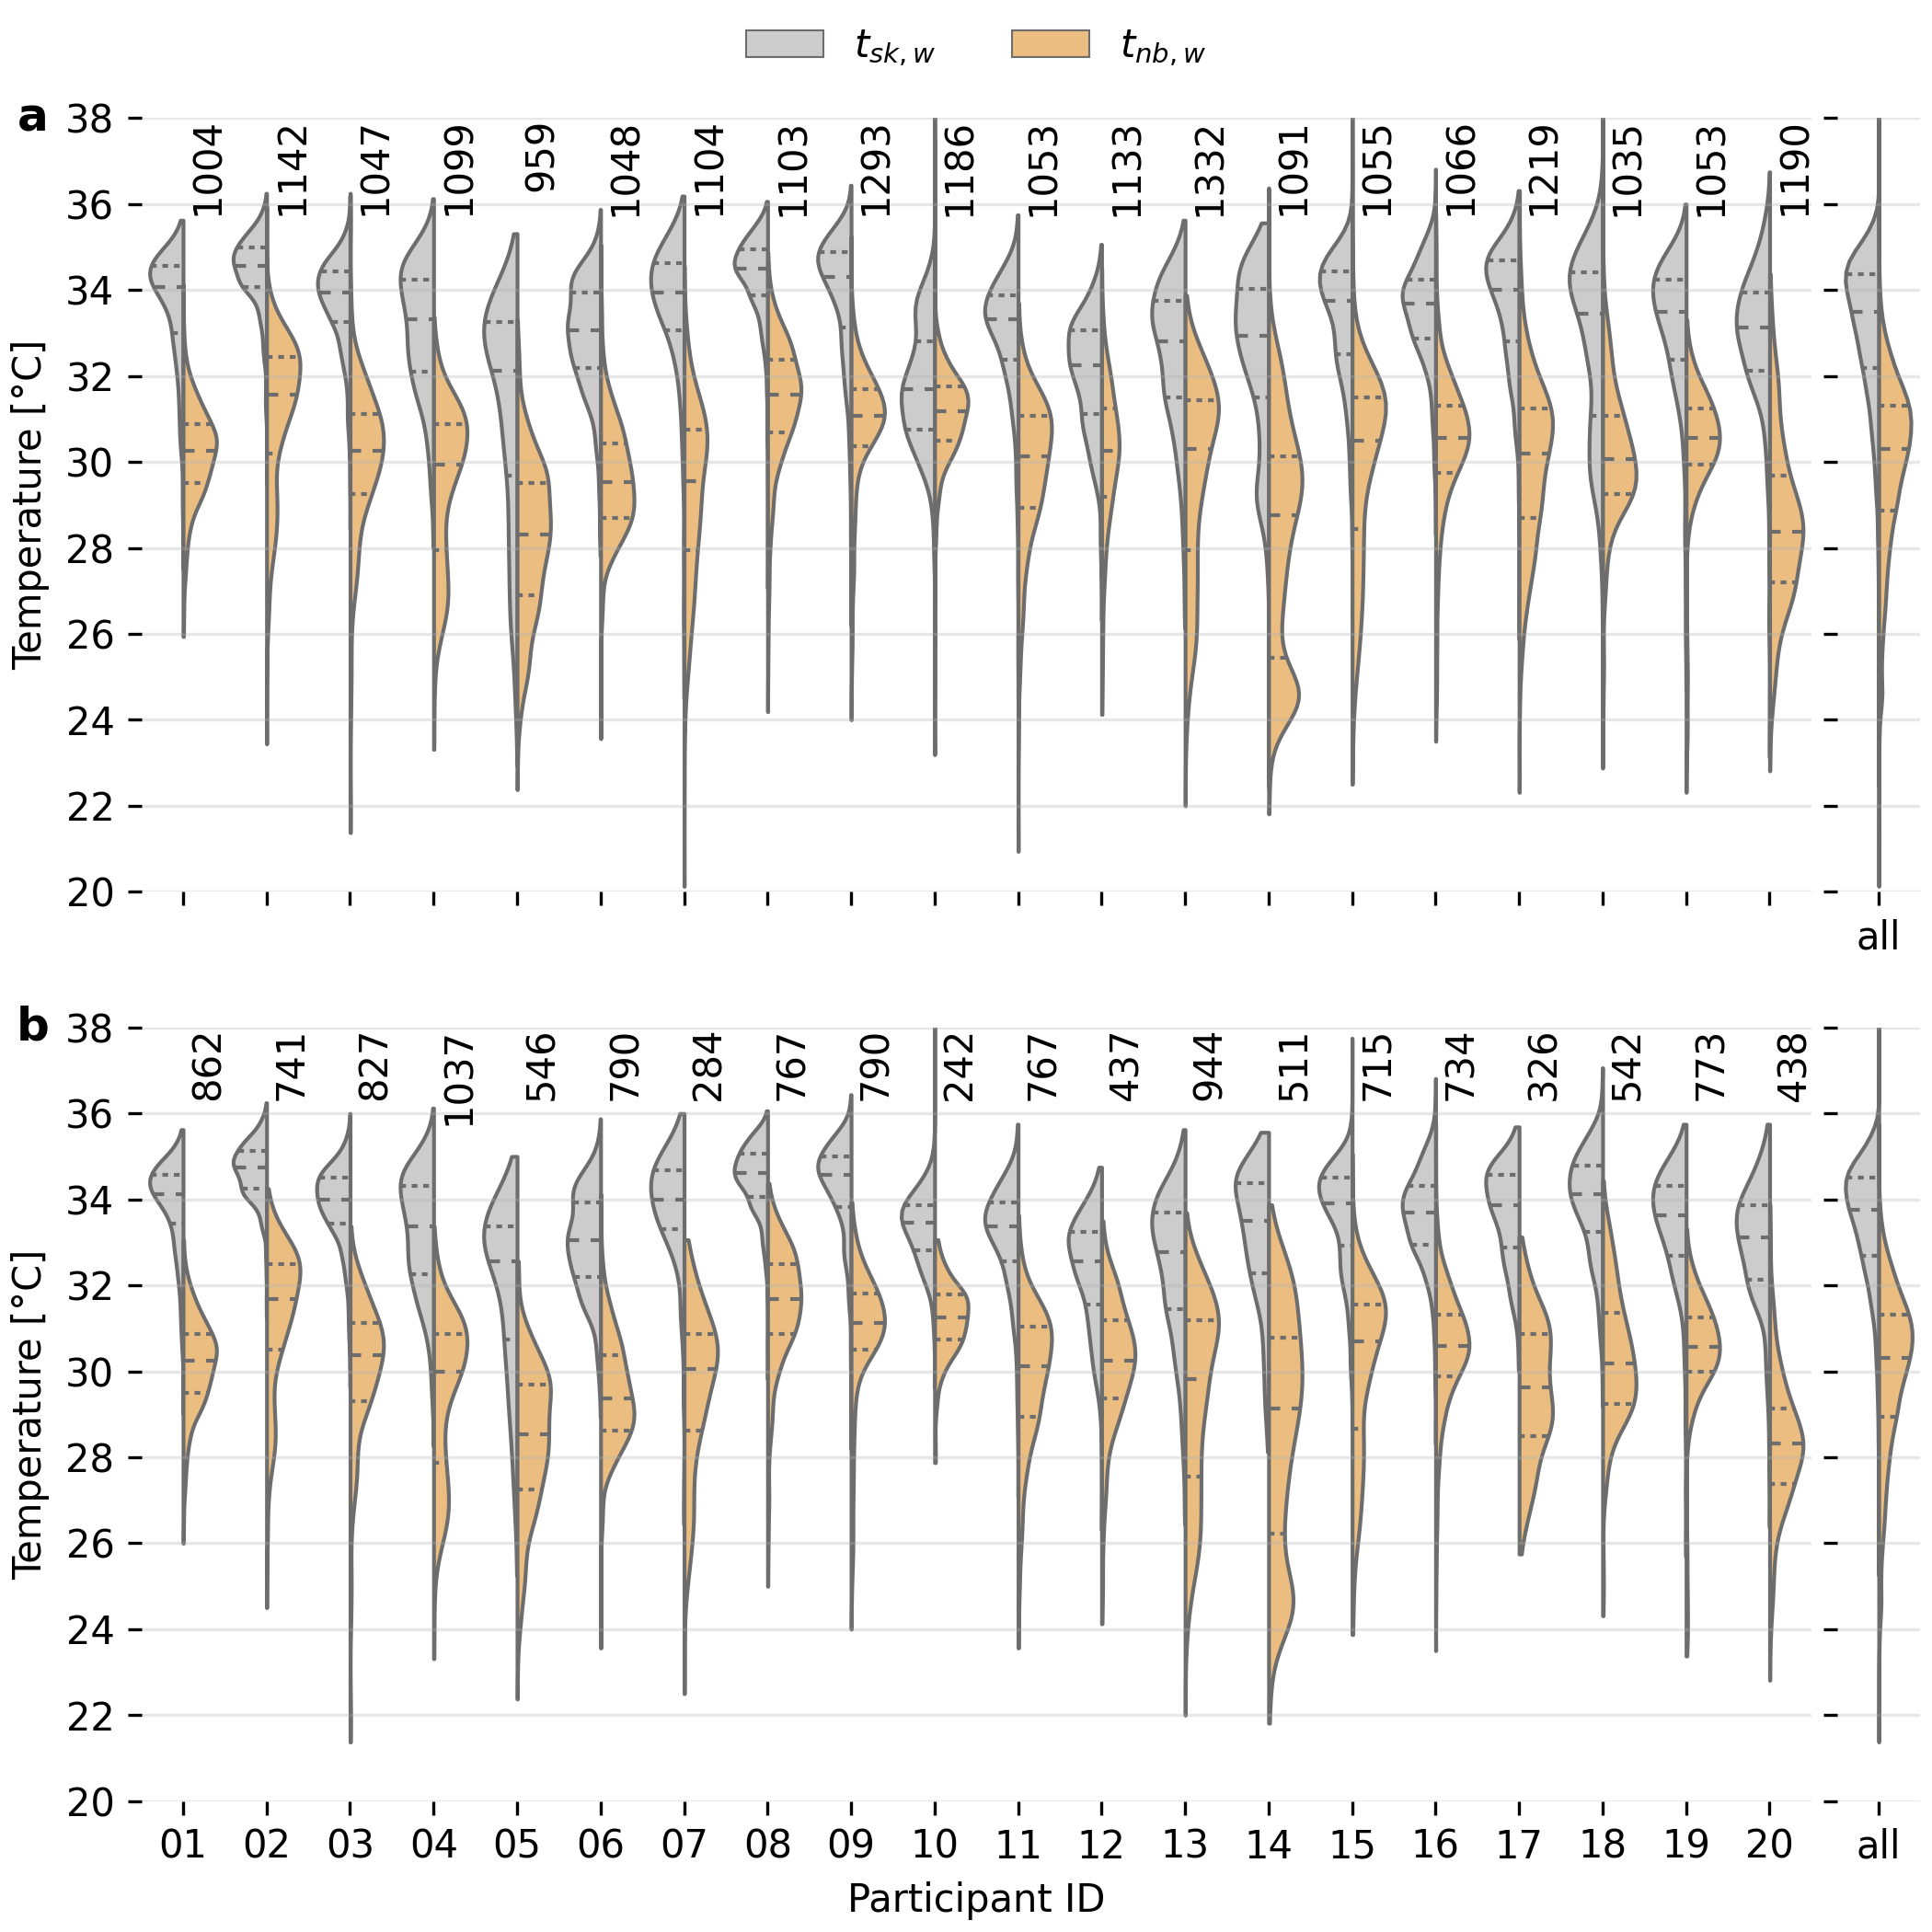
\includegraphics[width=\linewidth,height=\textheight,keepaspectratio]{figures/figure_3}
     \end{center}
     \caption{\Acf{t-sk-w} and \acf{t-nb} measured when the participants completed the \ac{rhrn} survey.
     Figure (a) shows all the data collected from the participants while Figure (b) shows the sub-set of the original dataset that was used in the data analysis.
     The inclusion criteria we used to filter the original dataset are detailed in Section\ref{subsec:datasetPreparationAndCleaning}.
     The number above each violin plot is the number of \ac{rhrn} surveys completed by each participant.
     }\label{fig:tmp_skin_nb_survey}
 \end{figure}
 
\begin{figure}[thb!]
    \begin{center}
        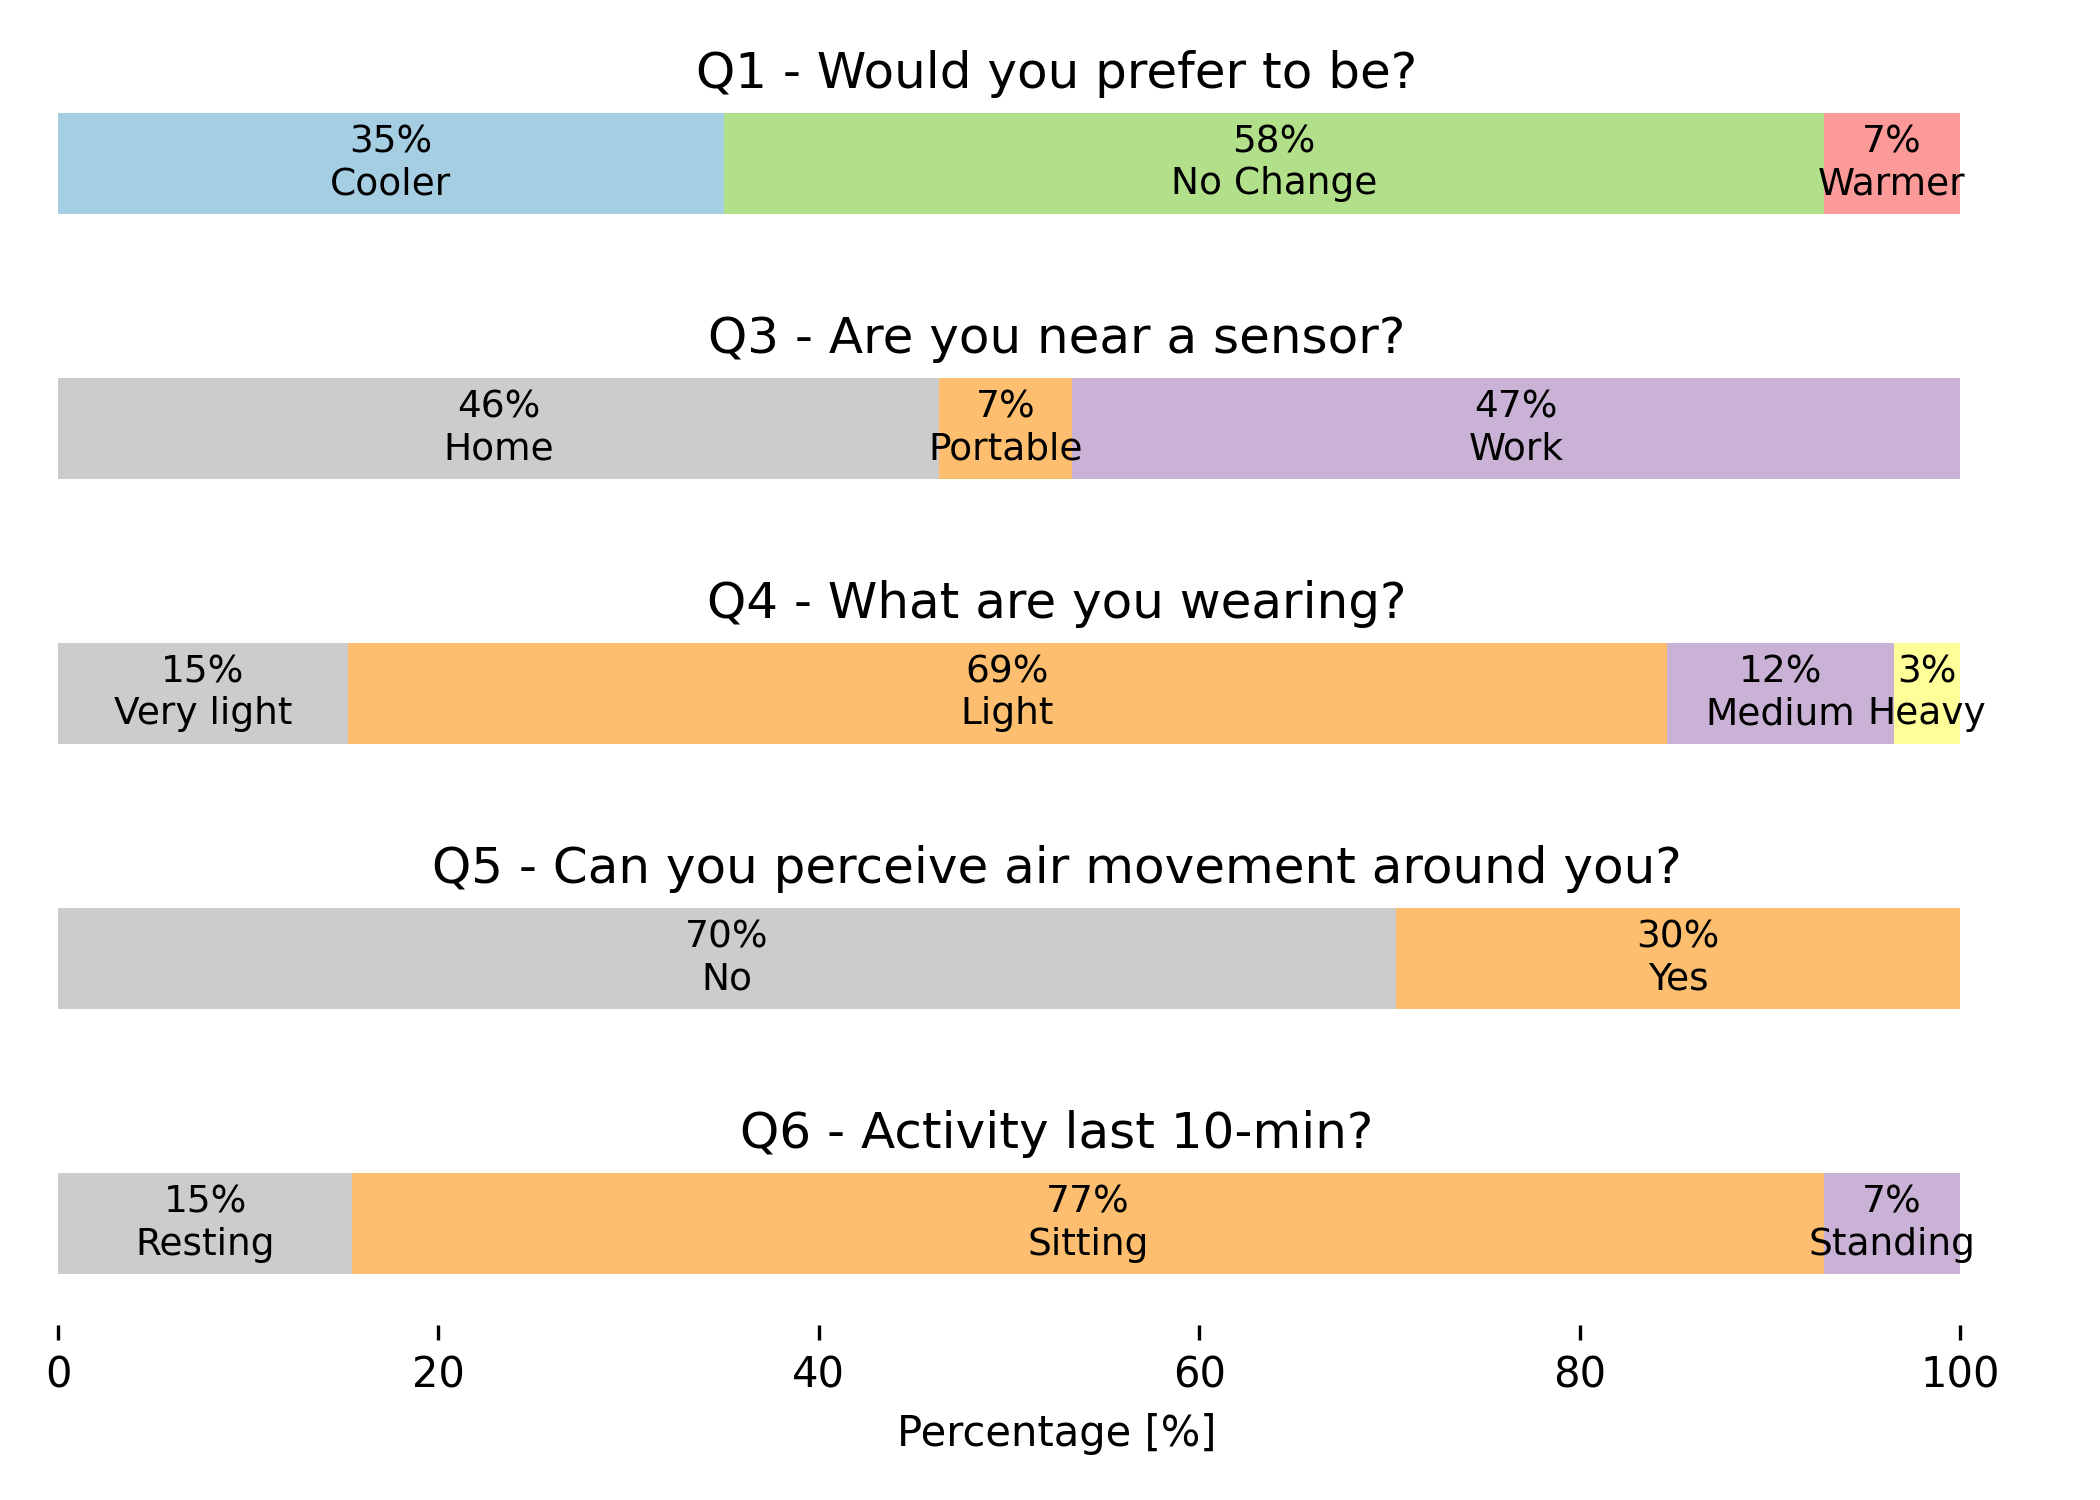
\includegraphics[width=\linewidth]{figures/figure_4}
    \end{center}
    \caption{Distribution of the answers provided by all the participants.}\label{fig:ans_distribution}
\end{figure}

\begin{figure}[thb!]
    \begin{center}
        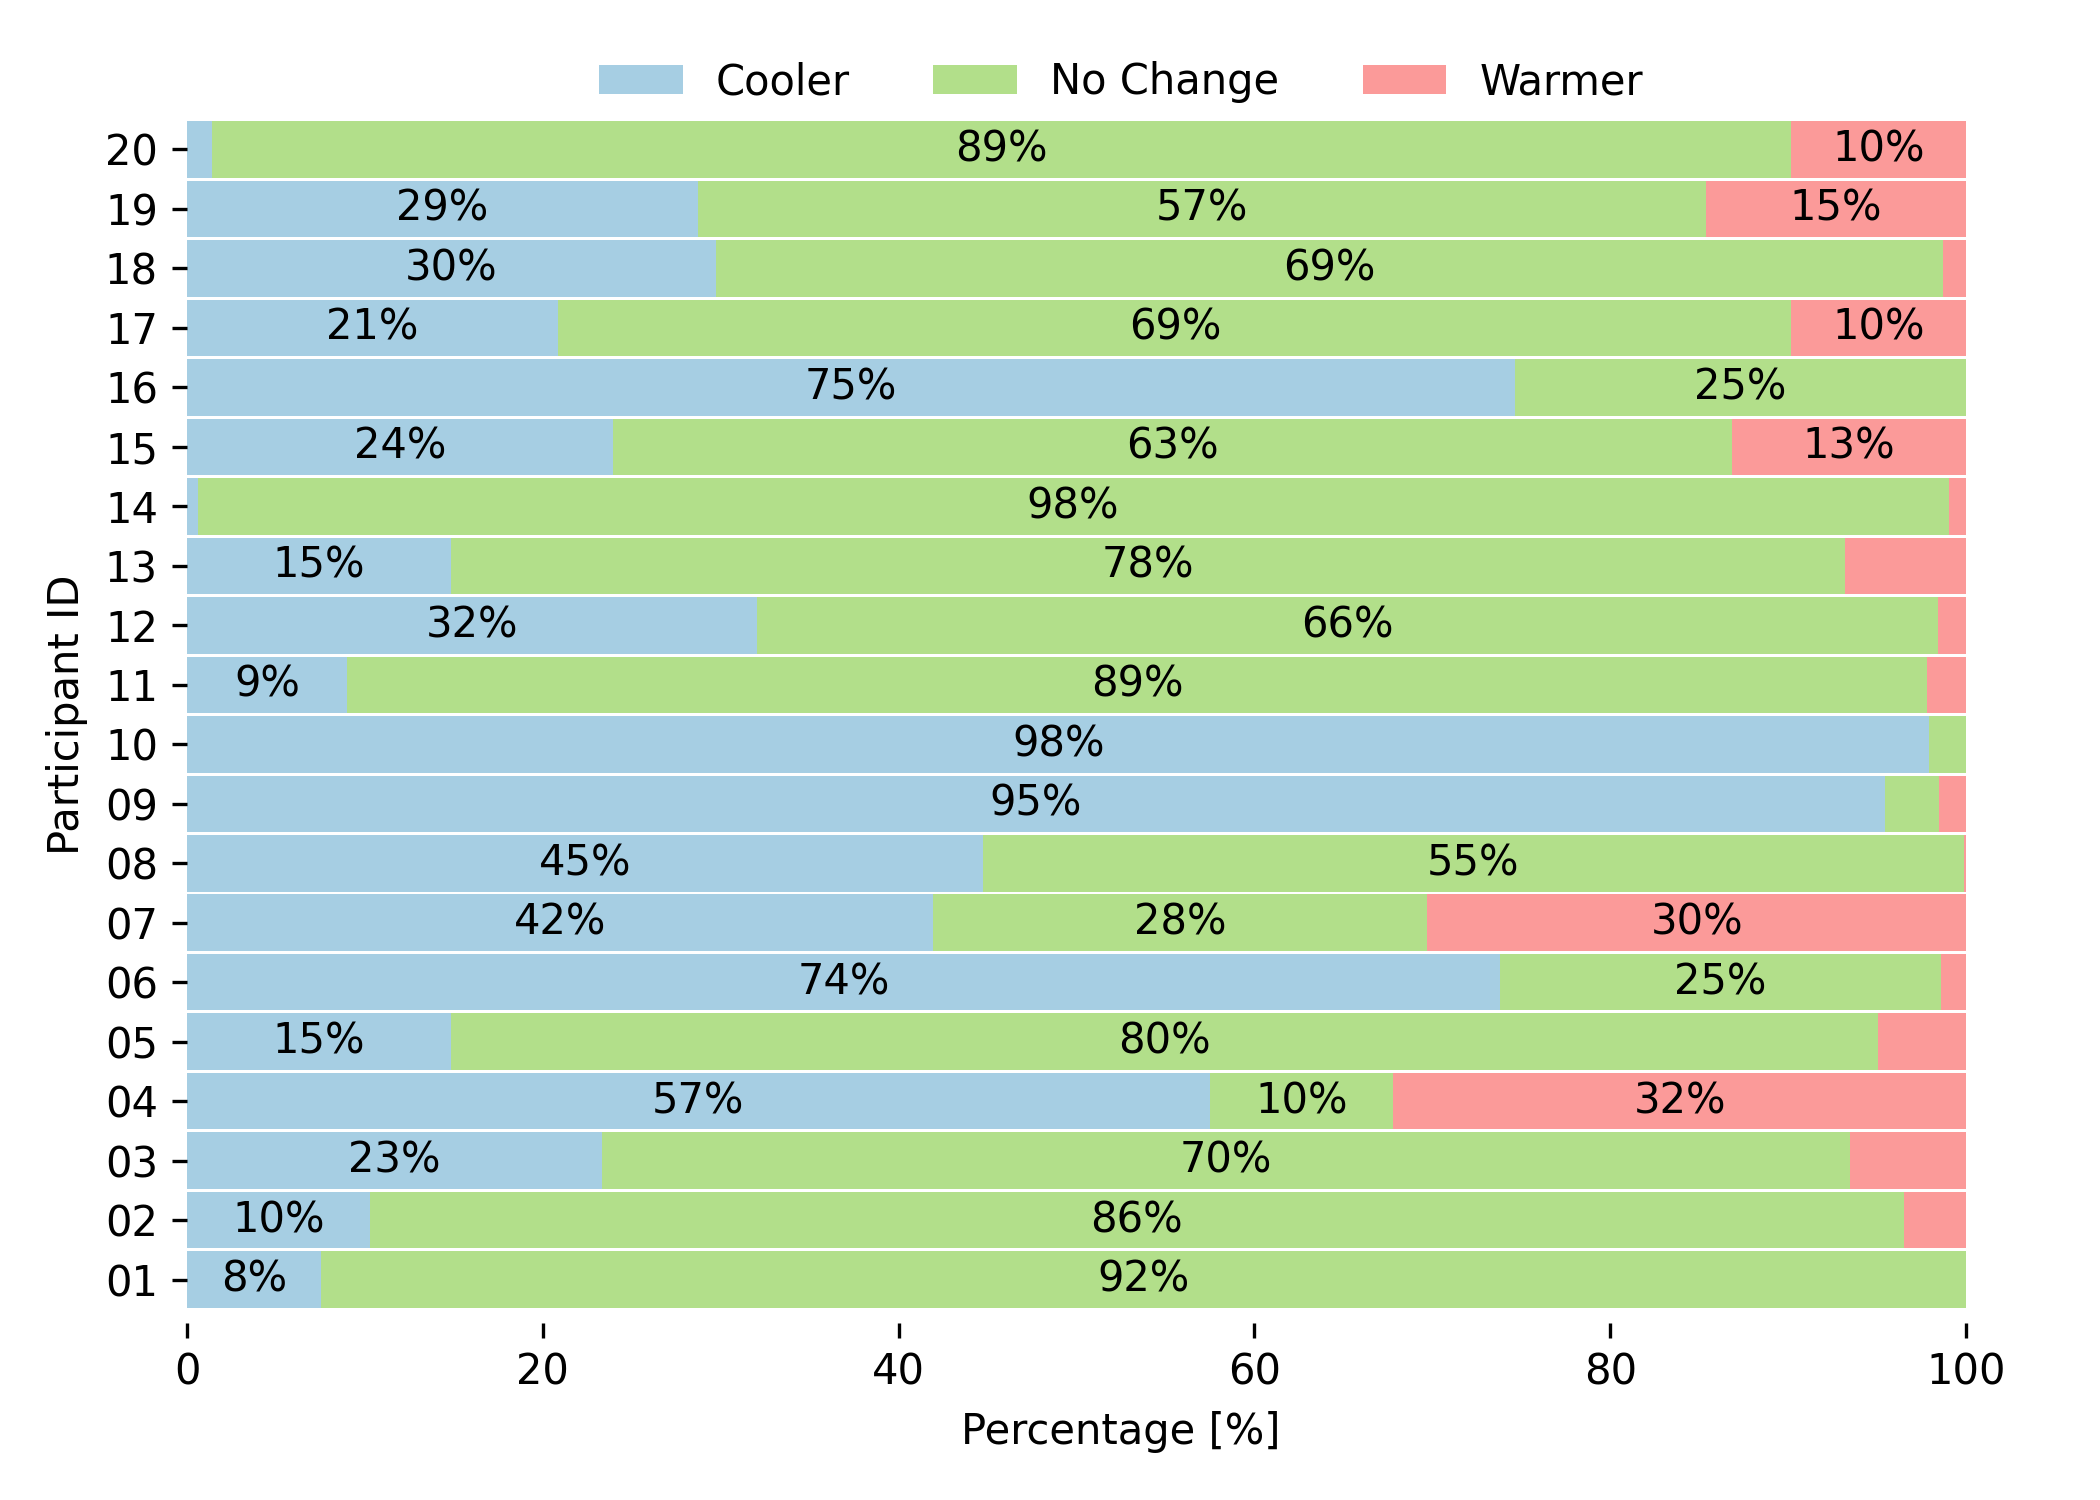
\includegraphics[width=\linewidth,height=\textheight,keepaspectratio]{figures/figure_5}
    \end{center}
    \caption{Distribution of the thermal preference responses (Q.1) provided by each participant throughout the study period.}\label{fig:thermal_by_userid}
\end{figure}
Most of the participants reported being involved in sedentary activities in \var{per_sitting}~\% of the cases.
Participants perceived air movement only less than \var{per_air_movement}~\% of the time, and \var{per_clo_light}~\% of them worn `Light' clothes.

To better depict how participants perceive their thermal environment, in Figure~\ref{fig:thermal_by_userid} we plotted the distribution of the thermal preference votes (Q.1) grouped by participant.
While the great majority voted `No Change,' two wanted to be `Cooler' more than 90~\% of the time.
Even if participants had similar distributions of thermal preference votes, such as participants 05 and 13, they might have different thermal comfort needs, requirements, and preferences.
This situation can be explained by the fact that the participants wore different clothes, engaged in different activities, and were exposed to different environmental conditions.
The values of \ac{t-db} recorded when a participant completed the survey are shown in Figure~\ref{fig:tmp_env_survey}.
The Figure also depicts the outdoor temperature measured in Singapore during the entire study period.
Singapore is characterized by a tropically hot and humid climate with limited seasonal temperature variation.
Temperature variation mainly occurs intra-day.

 \begin{figure}[thb!]
     \begin{center}
        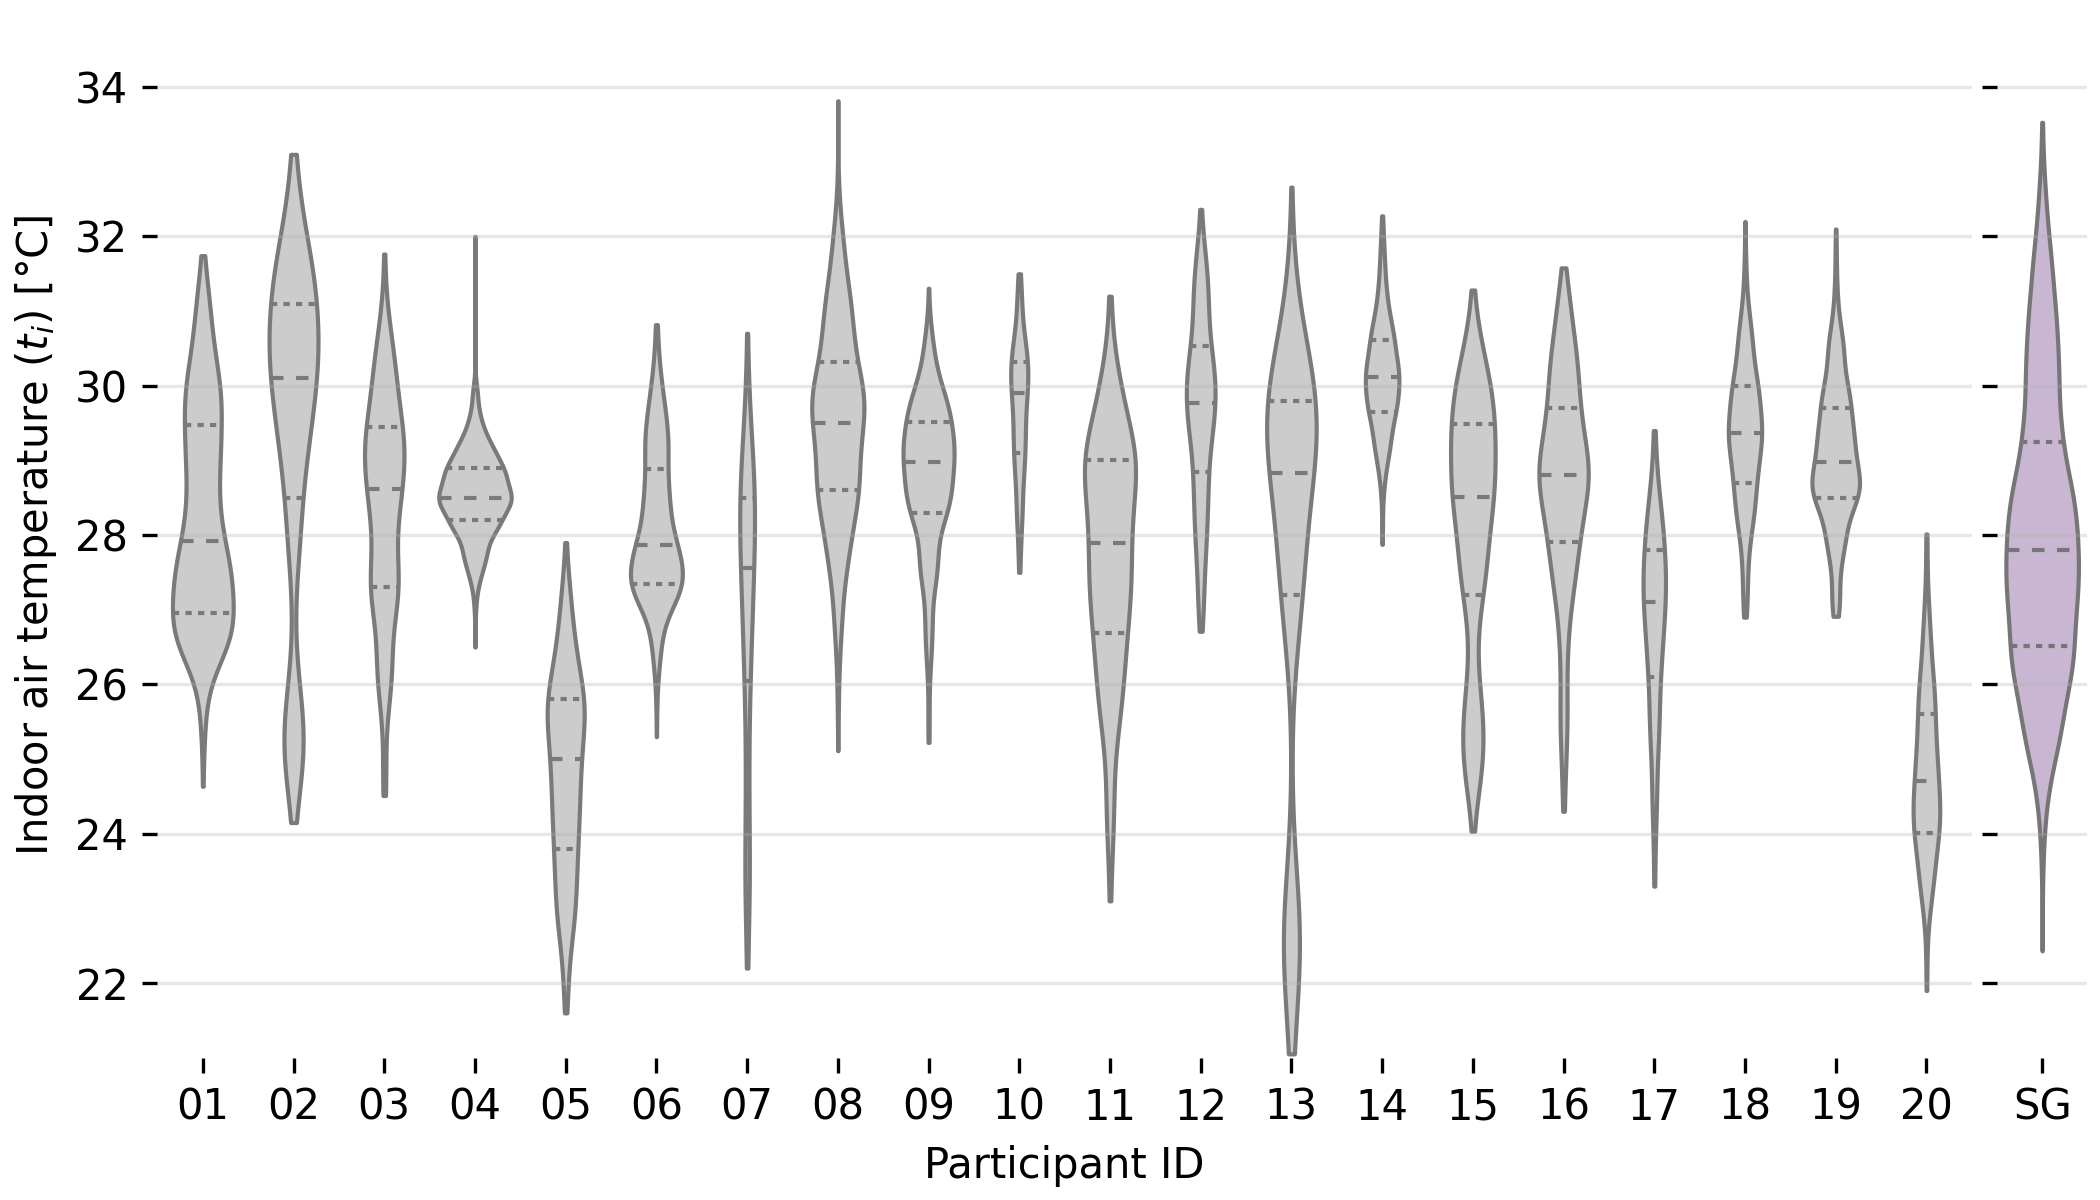
\includegraphics[width=\linewidth,height=\textheight,keepaspectratio]{figures/figure_6}
     \end{center}
     \caption{\Acf{t-db} measured when participants completed the \ac{rhrn} survey.
     Data have been grouped by participant.
     The last violin plot (purple) shows the average outdoor air temperature measured in Singapore (SG) throughout the whole duration of the study.}\label{fig:tmp_env_survey}
 \end{figure}

\begin{figure}[thb!]
    \begin{center}
        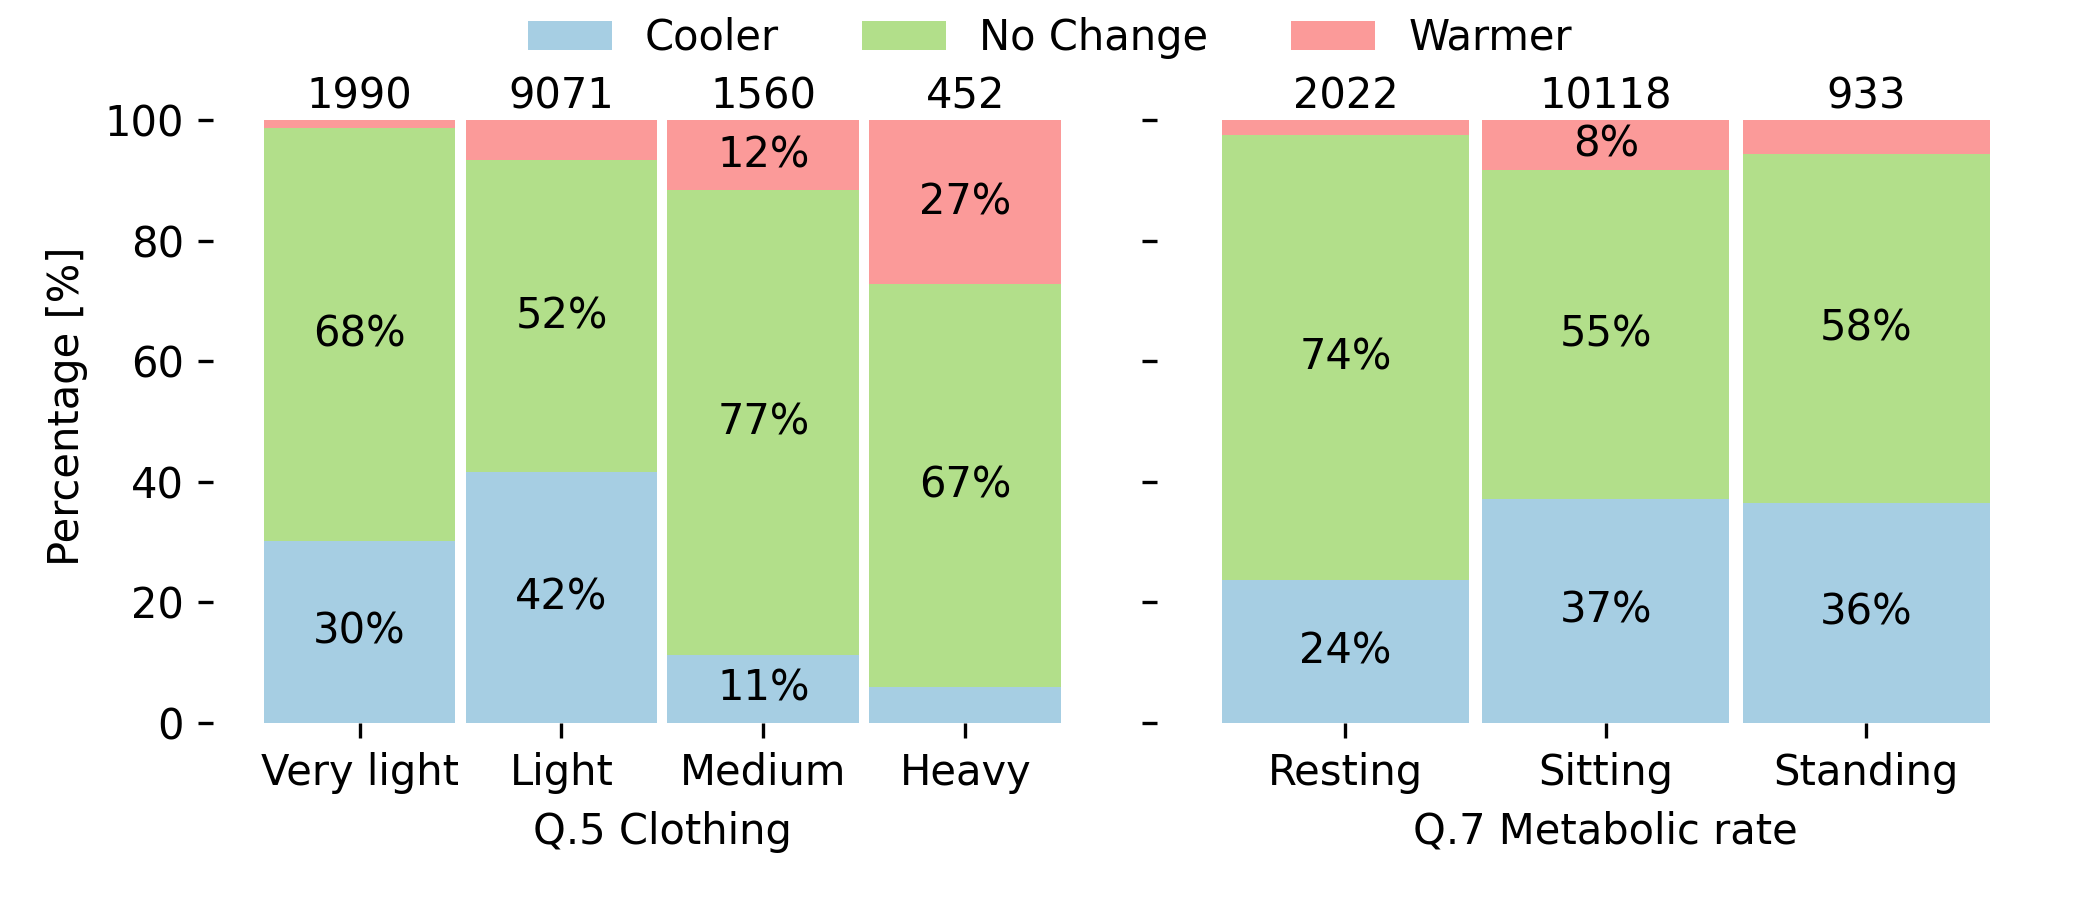
\includegraphics[width=\linewidth,height=\textheight,keepaspectratio]{figures/figure_7}
    \end{center}
    \caption{Distribution of the thermal preference responses (Q.1) provided by all participants throughout the study period grouped by their reported clothing insulation (Q.4) and metabolic rate (Q.6).
    The number above each bar shows the total number of responses collected for that specific answer.}\label{fig:tpv_by_cat}
\end{figure}

The thermal preference votes grouped by the self-reported clothing and metabolic rates are shown in Figure~\ref{fig:tpv_by_cat}.
Participants actively adjusted clothing to improve their thermal comfort.
They wore `Very light' clothes to compensate for warm indoor air temperatures.
Participants also actively increased their clothing levels when exposed to temperatures they deemed to be `Cold.'
Thus \var{heavy_clo_no_change}~\% of participants wearing `Heavy' clothing felt comfortable.
Wearing more clothes alone did not always suffice to compensate for cold indoor conditions.
Overcooling indoors was the leading cause that \var{heavy_clo_warmer}~\% of them wanted to be `Warmer', even though participants wore `Heavy' clothing in a tropical climate.
This is a common issue for buildings located in the tropics~\cite{Sekhar2016}.
Overcooling does not only negatively impact building energy consumption, but in the tropics has also been shown to worsen occupants' cognitive performance~\cite{Schiavon2016}.
Approximately \var{met_resting_no_change}~\% of the participants who reported to be `Resting' voted `No Change' in question Q.1.

\subsection{Thermal preference personal comfort models}
The prediction accuracy of the personal comfort model we developed is depicted in Figure~\ref{fig:boxen_comp_metrics_thermal}.
The Figure shows the F1-micro scores for the three sets of variables grouped by the supervised machine learning model we used to train the personal comfort models.
We also report the PMV model results.
\begin{figure}
    \begin{center}
        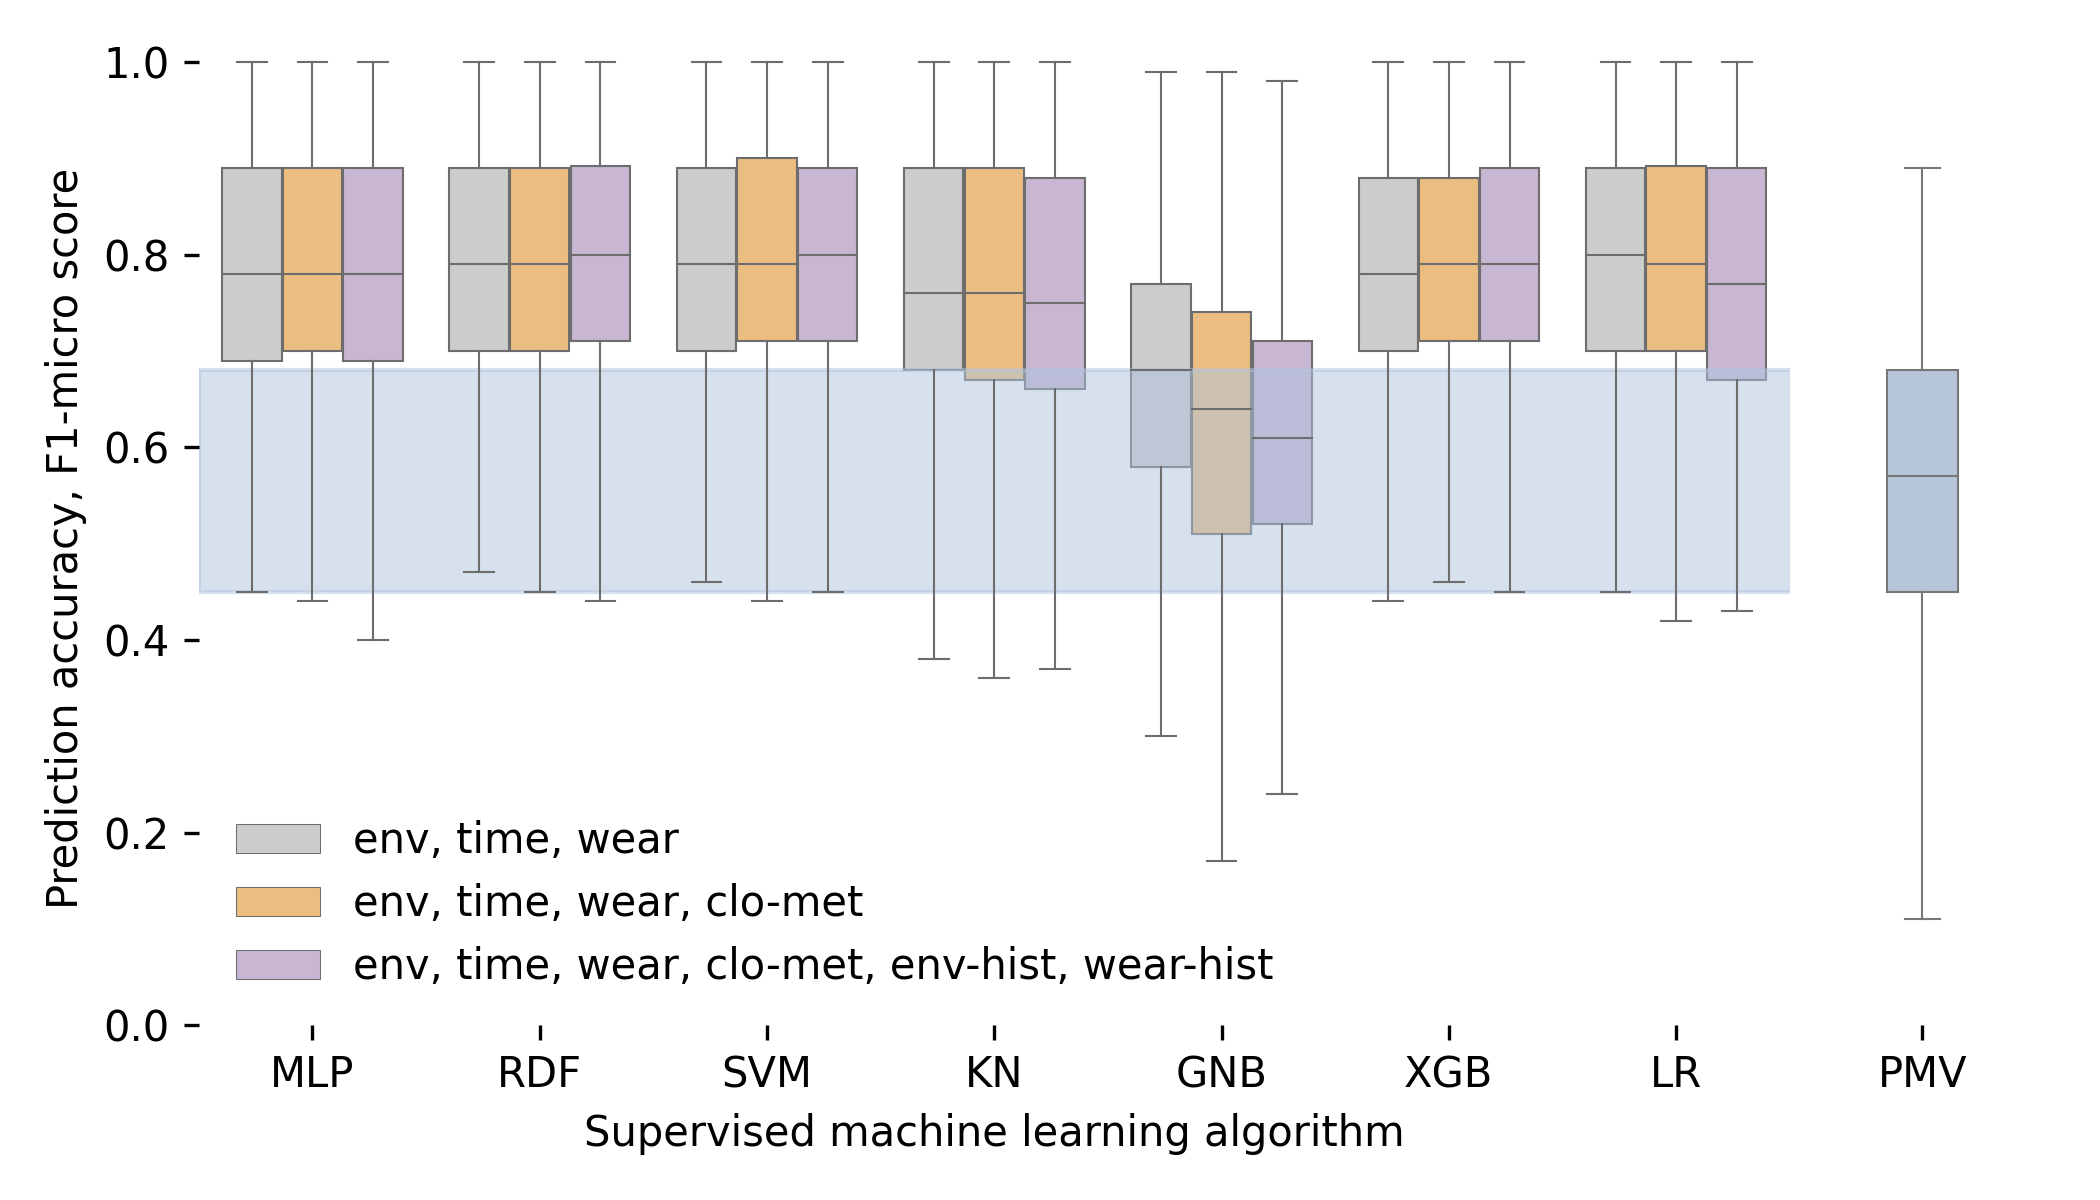
\includegraphics[width=\linewidth,height=\textheight,keepaspectratio]{figures/figure_8}
    \end{center}
    \caption{F1-micro scores for the thermal preference personal comfort models determined using the full dataset for each participant over 100 iterations.
    The light blue shaded area depicts the interquartile range for the \ac{pmv} model. We used the following abbreviations in the Figure: Multi-Layer Perceptron (MLP), Random Forest (RDF), Support Vector Machine (SVM), K-Nearest Neighbors (KN), Gaussian Naive Bayes (GNB), Extreme Gradient Boosting (XGB), Logistic Regression (LR).}\label{fig:boxen_comp_metrics_thermal}
\end{figure}
The prediction accuracy of all the personal comfort models developed with the supervised machine learning algorithms was significantly ($p < 0.01$) and substantially (excluding Extreme Gradient Boosting) higher ($\approx37\%$) than the results obtained from the \ac{pmv} model.
In our study, we only qualitatively logged clothing levels and metabolic rates, and we did not measure airspeed as detailed in the Methodology Section.
Hence, we do not have sufficient evidence to prove that the \ac{pmv} has low prediction accuracy.
We simply report the results of the \ac{pmv} to provide a benchmark to show the increase in accuracy that personal comfort models can achieve.
This is, however, a common issue in real buildings, hence these values must also be assumed to calculate the \ac{pmv}.

One of the main objectives of this study was to determine how different sub-sets of variables would affect the accuracy of the models.
Adding an increased number of variables to the model did not always improve its accuracy.
In some cases, it had the opposite effect and led to a decreased F1-micro score.
Similar results were also obtained in previous studies~\cite{Liu2019a}.
This can be partially explained because participants completed surveys in near-steady-state conditions.
Hence, including historical data is not always beneficial.
Moreover, self-reported clothing and activity may not have accurately enough represented participants' actual clothing ensembles or metabolic rate since their selection was limited to four choices.
This is a positive result since in a real-life scenario we would not have access to this information.

The distribution of the F1-micro scores was significantly different when we compared the results of the following models Extreme Gradient Boosting, \ac{svm}, \gls{rdf}, \gls{lr}, \gls{mlp} using different variable sets.
However, the significant increase in model complexity would not justify the modest increase in prediction accuracy in most practical applications.
On average, training one model once with the full variable set for each 20 users resulted took 83, 6, 620, 11, and 67 seconds for Extreme Gradient Boosting, \ac{svm}, \gls{rdf}, \gls{lr}, \gls{mlp} models, respectively.
We consequently decided to present only the results from the \ac{svm} model trained with the \textit{environmental -- wearable -- time} independent sets of variables in Figure~\ref{fig:thermal_f1_micro_env_sma_oth} and \ref{fig:shapely_summary}.
Firstly, because the \ac{svm} model is less computationally intensive to train and secondly because it is a linear model, hence it is better suited to predict thermal preference which is an ordinal variable.
We are providing supporting evidence on this in the Discussion Section.
Linear models use a multidimensional hyperplane to classify the data, this may lead to lower prediction accuracy if compared with non-linear models.
Nevertheless, linear models ensure that as \ac{t-db} increases, all other variables being fixed, the prediction does not switch back and forth between `Warmer', `No Change', and `Cooler'.
This issue is particularly relevant when personal comfort models are used in real-life applications to operate buildings.
Non-linear model predictions may be the cause of instabilities in the HVAC controller and limit the use of personal comfort models to control buildings. 

\subsubsection{Influence of data size on prediction power}
Figure~\ref{fig:thermal_f1_micro_env_sma_oth}~a depicts how the F1-micro score varies as a function of the number of training data points for each participant.
The Figure also shows the F1 mean score (black line) and its standard deviation (shaded area) across all participants.
\begin{figure}
\centering
    \begin{subfigure}{\textwidth}
        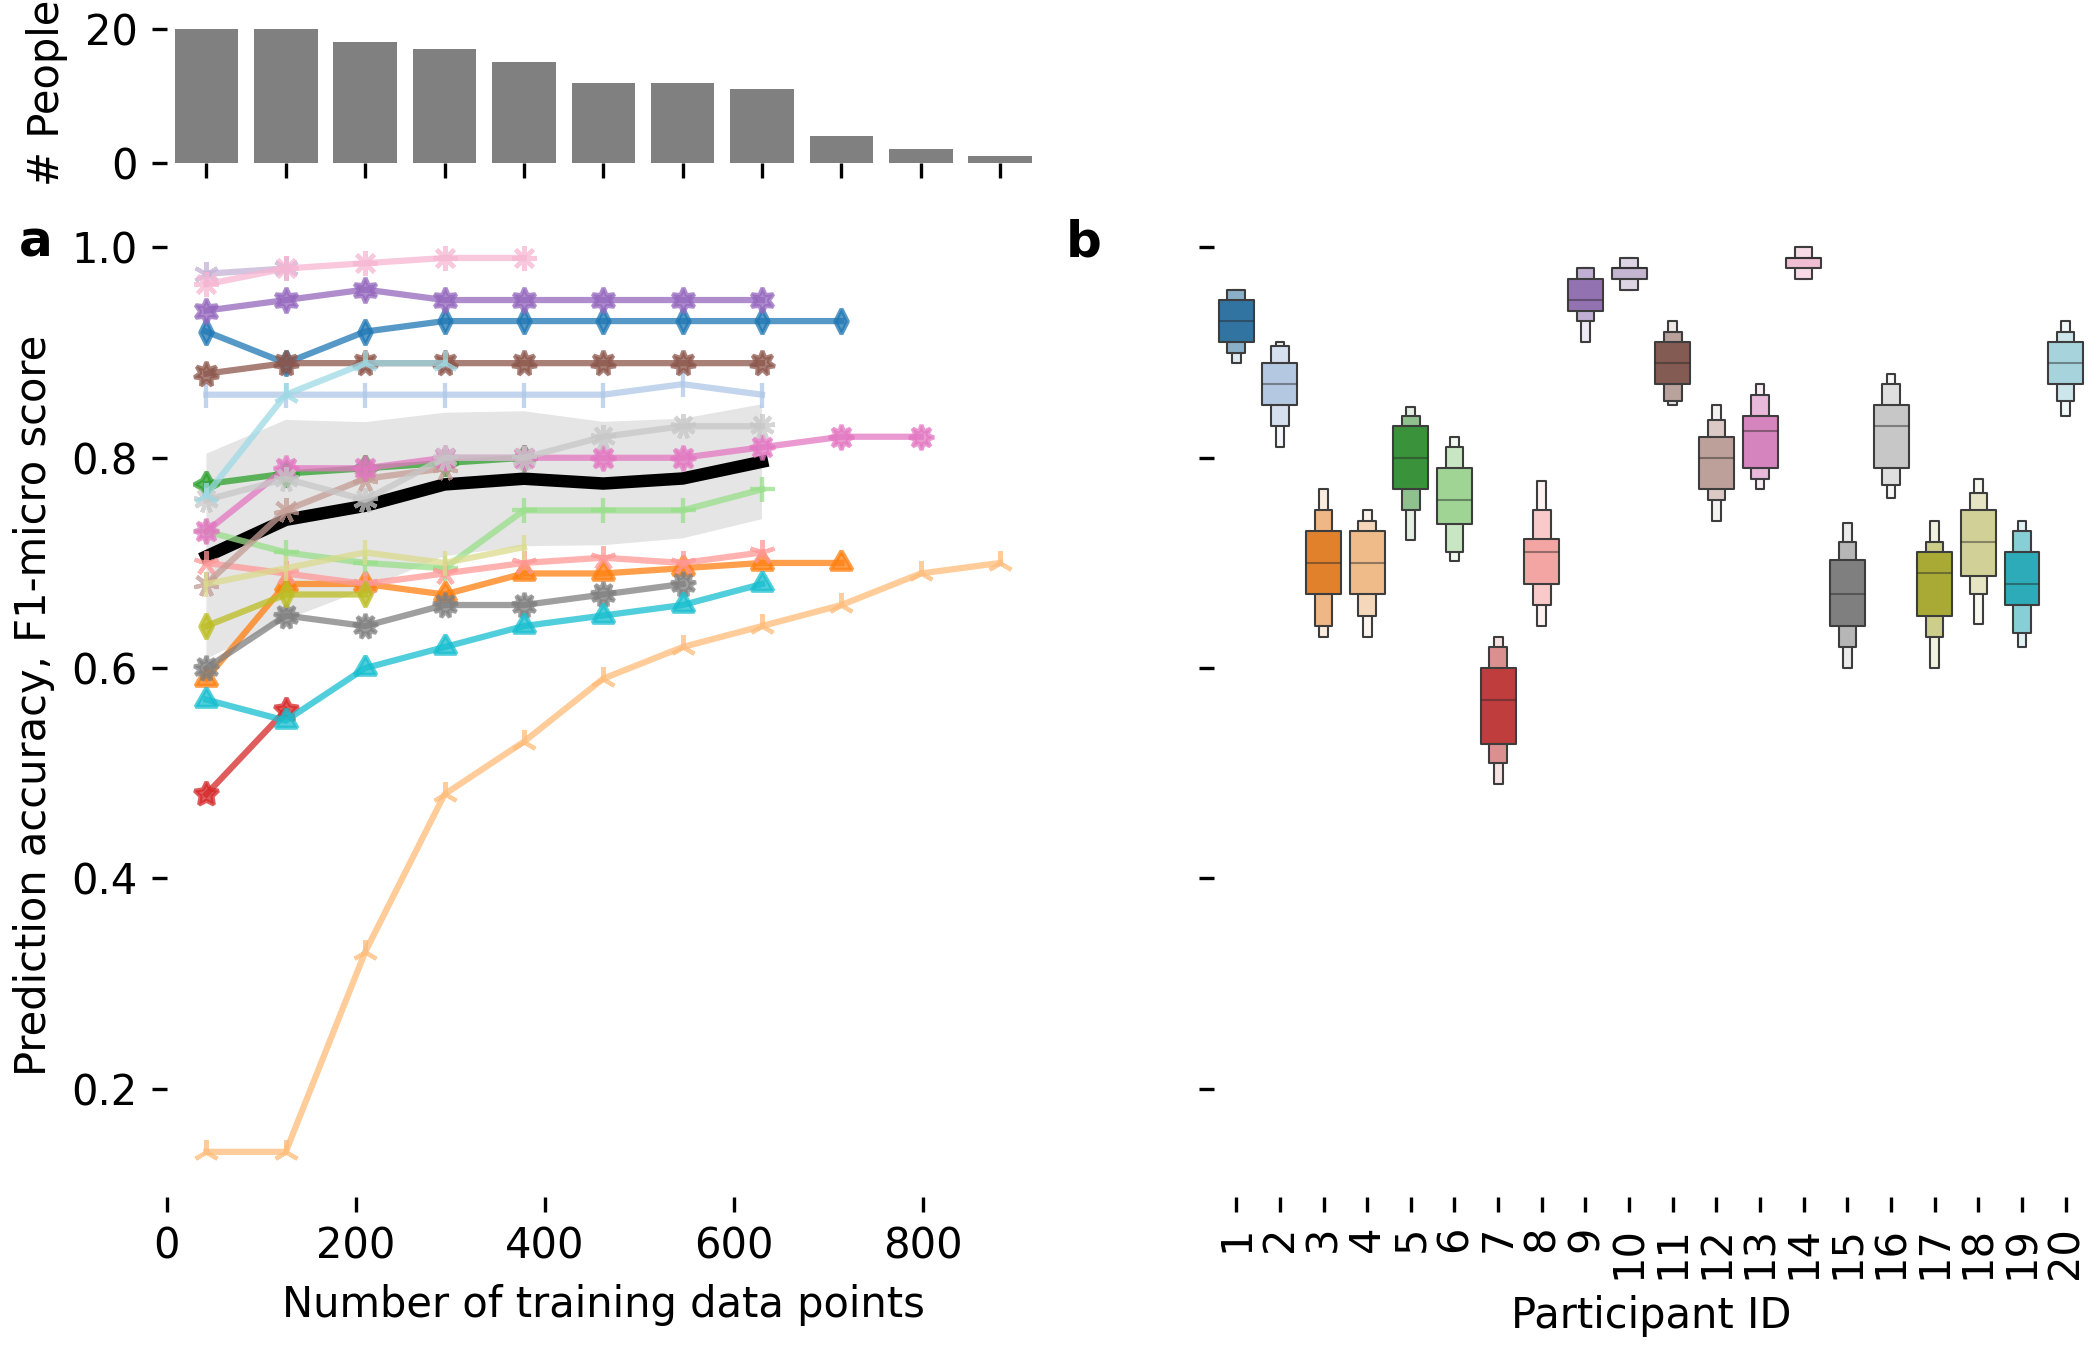
\includegraphics[width=\linewidth,height=\textheight,keepaspectratio]{figures/figure_9}
        \caption{\acf{svm}}
    \end{subfigure}
    \caption{F1-micro scores for the thermal preference personal comfort models determined using the \acf{svm} algorithm.
    Figure (a) shows the mean F1-micro score for each participant, as well as the mean score (black line) and standard deviation across (shaded area) the whole study sample.
    The markers show the participant's mean F1-micro scores calculated by averaging the mean scores obtained across the 100 iterations, for that specific number of training data points.
    A different number of valid surveys were completed by different participants.
    The bar plot, in Figure (a) over the chart, shows the number of answers that were used to calculate the sample mean score and the respective standard deviation.
    Figure (b) shows all the F1-micro scores determined using the full dataset for each participant over 100 iterations.}\label{fig:thermal_f1_micro_env_sma_oth}
\end{figure}
The sample average accuracy mean score plateaued at around $\approx$~300 data points.
This suggests that this may be the optimal number of points we may need to collect when training personalized comfort models.
It should be noted that there was high variability in when the curve plateaued for each individual.
This is due to the inherited differences across personal preferences of subjects and the conditions they were exposed to.
Figure~\ref{fig:thermal_f1_micro_env_sma_oth}~b shows the overall accuracy of each personal comfort model over the 100 iterations.
It can be observed that each personal comfort model converged to a stable value across all 100 iterations.
The standard deviation of all 20 personal comfort models over all 100 iterations was similar across different participants, with a mean value of 0.035 and a standard deviation of 0.011.
The same cannot be said about the overall accuracy of each personal comfort model, where the median F1 score for participant 14 was 0.99 while for participant 7 was 0.56.
This, in other words, means that not all personal comfort models performed equally.
Some almost always correctly predicted the thermal preference vote reported by the participants, while others had a significantly lower accuracy.

\subsubsection{Importance of independent variables}
The absolute mean \gls{shap} values across all six best-performing supervised machine learning models are shown in Figure~\ref{fig:shapely_summary}.
Sub-variables groups defined in the Section~\ref{subsubsec:feature-selection} are color-coded.
While \acf{t-db}, \acf{t-nb}, \acf{hr}, \acf{t-sk-w}, and \acf{w-i} contributed the most to the models' final predictions, we observed a significant difference of \gls{shap} values between different participants and across different models.
In Figure~A.3 we report the mean \gls{shap} values across all participants for each supervised machine learning model.
A detailed discussion of these results is presented in Section~\ref{subsec:features}.
\begin{figure}
    \begin{center}
        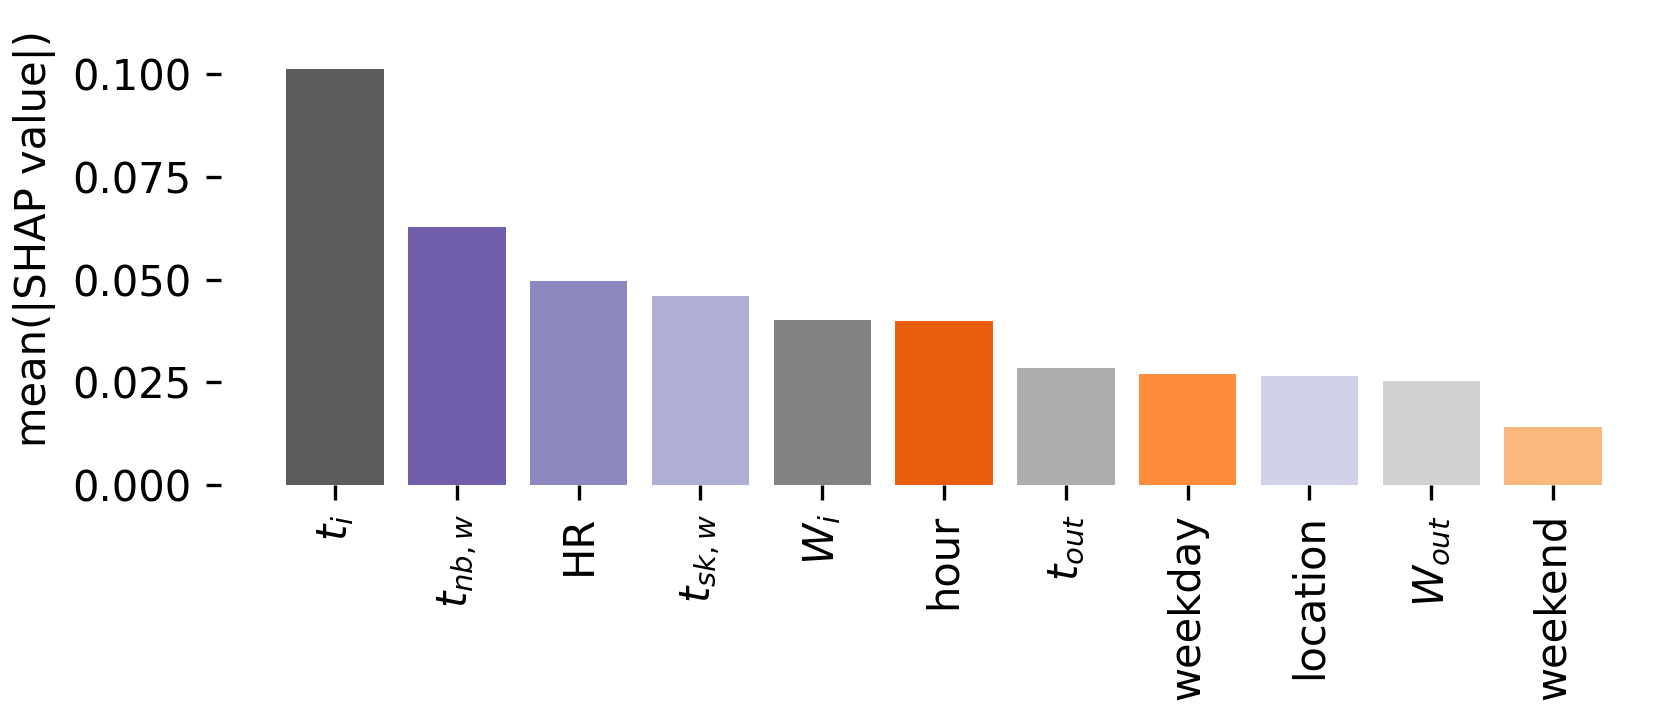
\includegraphics[width=\linewidth,height=\textheight,keepaspectratio]{figures/figure_10}
    \end{center}
    \caption{Absolute mean \gls{shap} value of the six best performing supervised machine learning models.
    Variables are color-coded, \emph{environmental} -- using shades of gray, \emph{wearable} -- using shades of purple, and \emph{time} -- using shades of orange.
    Where $t_{out}$ stands for outdoor air temperature, and $W_{out}$ stands for humidity ratio outdoors.}\label{fig:shapely_summary}
\end{figure}